\section{B. 던전 지도}

\begin{frame} % No title at first slide
    \sectiontitle{B}{던전 지도}
    \sectionmeta{
        \texttt{two\_pointer}\\
        출제진 의도 -- \textbf{\color{acgold}Easy}
    }
    \begin{itemize}
        \item 제출 611번, 정답 93팀 (정답률 15.38\%)
        \item 처음 푼 팀: \textbf{아뇨, 뚱인데요?} (ㅎㅎ;;, ㅈㅅ.., ㅋㅋ!!), 25분
        \item 출제자: \texttt{kdh9949}
    \end{itemize}
\end{frame}

\begin{frame}{\textbf{B}. 던전 지도}
    \begin{itemize}
        \item 보스 방에서부터 거꾸로 간다고 생각해 봅시다.
        \item DFS를 수행하면 \complexity{NM} 에 할 수 있을 것 같습니다.
        \item 물론 그렇게 문제가 호락호락하지 않습니다. $N$과 $M$이 20만씩이나 됩니다.
    \end{itemize}
\end{frame}

\begin{frame}{\textbf{B}. 던전 지도}
    \vspace{8pt}
    \begin{itemize}
        \item 지도가 행 단위로 이루어져 있으니, 마지막 행부터 순서대로 살펴봅시다.
        \item 마지막 행의 경우, 보스 방을 제외하고 가장 오른쪽에 있는 \texttt{U} 바로 오른쪽 방부터 보스 방까지, 즉 어떤 \textbf{구간} 내에 존재하는 방들이 보스 방에 도달할 수 있는 방이 됩니다.
    \end{itemize}
    \begin{center}
        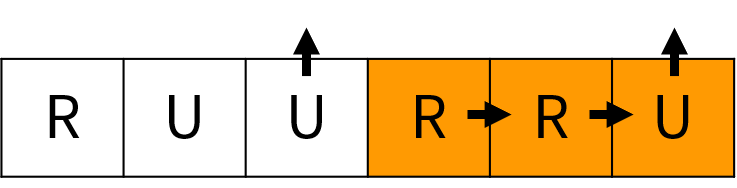
\includegraphics[width=0.4\linewidth]{../images/dungeon-map/b-lastrow.png}
    \end{center}
    \begin{itemize}
        \item 그 아래 행에서도 보스 방에 도달 가능한 방들이 구간으로 나타난다면 참 좋을 것 같은데.. 과연 그럴까요?
    \end{itemize}
\end{frame}

\begin{frame}{\textbf{B}. 던전 지도}
    \vspace{14pt}
    \begin{itemize}
        \item 각 행에 대해, 왼쪽에서 $x$번째에 있는 방의 좌표를 $x$라고 합시다.
        \item 현재 행의 좌표 $x$에서 시작했을 때 처음 도달하는 바로 위 행의 좌표를 $n(x)$라고 합시다. \\
        (바로 위 행에 도달하지 않는다면 $M+1$로 정의)
        \item 두 좌표 $a < b$에 대해 $n(a) \le n(b)$ 입니다. 또한, (현재 행에서 $a$가 보스 방에 도달하는 좌표인 것)과 (바로 위 행에서 $n(a)$가 보스 방에 도달하는 좌표인 것)은 동치입니다.
    \end{itemize}
    \begin{center}
        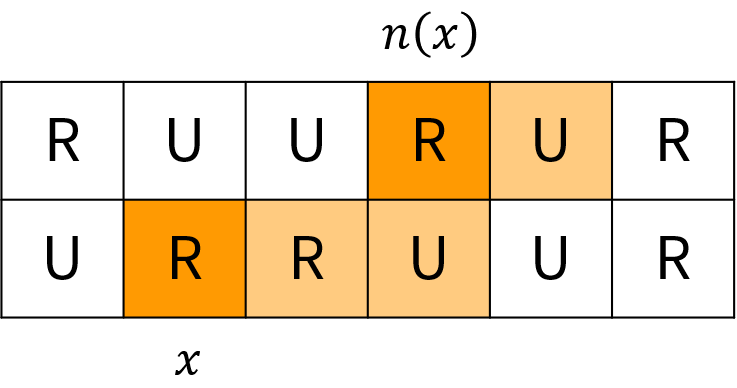
\includegraphics[width=0.35\linewidth]{../images/dungeon-map/b-basic.png}
    \end{center}
\end{frame}
        
\begin{frame}{\textbf{B}. 던전 지도}
    \vspace{14pt}
    \begin{itemize}
        \item 어떤 행에 대해, 바로 위 행에서 [$s, e$] 구간이 보스 방에 도달하는 구간이라고 합시다.
        \item 세 좌표 $u < v < w$에 대해 $u$와 $w$가 둘 다 보스 방에 도달하는 좌표라고 해 봅시다.
        \item $n(u)$와 $n(w)$가 모두 [$s, e$] 구간에 속합니다. 따라서, $s \le n(u) \le n(v) \le n(w) \le e$이므로 $n(v)$ 역시 [$s, e$] 구간에 속하게 되고, $v$ 역시 보스 방에 도달하는 좌표가 됩니다. 즉, \textbf{각 행에서 보스 방에 도달하는 좌표는 구간으로 나타납니다.}
    \end{itemize}
    \begin{center}
        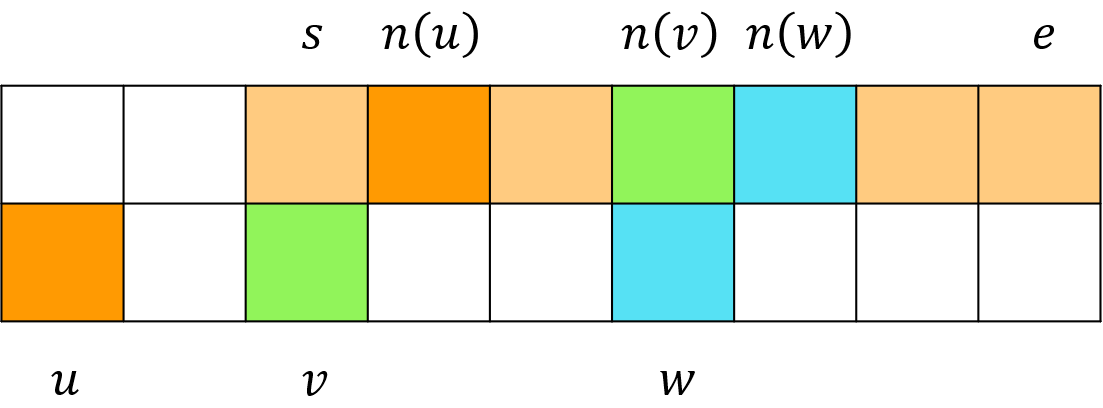
\includegraphics[width=0.5\linewidth]{../images/dungeon-map/b-proof.png}
    \end{center}
\end{frame}

\begin{frame}{\textbf{B}. 던전 지도}
    \vspace{14pt}
    \begin{itemize}
        \item 각 행에 대해 보스 방에 도달하는 좌표의 구간을 계산하여 그 길이를 모두 더하면 답이 됩니다.
        \item 바로 윗 행의 구간을 알 때, 현재 행의 구간은 어떻게 계산할까요?
        \item 좌표 $x$에 대해 ($y \le x$이고 해당 좌표에 적힌 글자가 \texttt{U}인 $y$) 중 최댓값을 $f(x)$라고 합시다.
        \item 바로 윗 행의 구간이 [$s, e$]라면, 현재 행에 해당하는 구간은 [$f(s-1)+1, f(e)$] 가 됩니다.
    \end{itemize}
    \begin{center}
        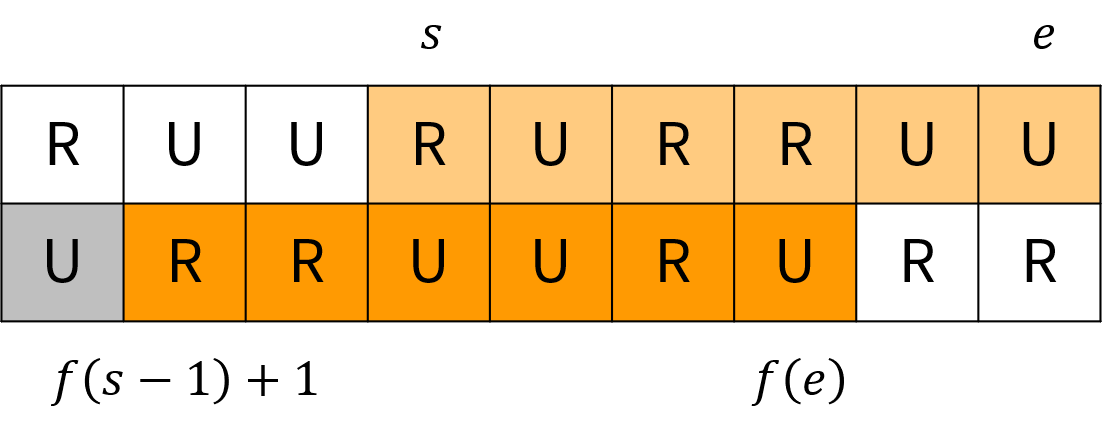
\includegraphics[width=0.5\linewidth]{../images/dungeon-map/b-calc.png}
    \end{center}
\end{frame}

\begin{frame}{\textbf{B}. 던전 지도}
    \begin{itemize}
        \item $f(s-1)+1 \le s$, $f(e) \le e$ 이므로 행을 하나씩 내려갈 때마다 구간의 양 끝점은 오른쪽으로 절대 이동하지 않습니다.
        \item 구간의 양 끝점 좌표를 하나씩 감소시키면서 $f(x)$ 값을 계산하면 알고리즘 전체 작동 시간이 \complexity{N+M}이 됩니다.
        \begin{itemize}
            \item 이 테크닉을 Two pointer 내지는 Inchworm이라고 부릅니다.
        \end{itemize}
        \item 입력을 받아야 하니 총 시간복잡도는 \complexity{N+KM} 입니다.
    \end{itemize}
\end{frame}